%\documentclass[a4paper]{article}
\usepackage[utf8]{inputenc}
\usepackage[spanish, es-tabla, es-noshorthands]{babel}
\usepackage[table,xcdraw]{xcolor}
\usepackage[a4paper, footnotesep = 1cm, width=22cm, top=2.5cm, height=25cm, textwidth=20cm, textheight=25cm]{geometry}
%\geometry{showframe}

\usepackage{tikz}
\usepackage{amsmath}
\usepackage{amsfonts}
\usepackage{amssymb}
\usepackage{float}
\usepackage{graphicx}
\usepackage{caption}
\usepackage{subcaption}
\usepackage{multicol}
\usepackage{multirow}
\usepackage{wrapfig}
\setlength{\doublerulesep}{\arrayrulewidth}
\usepackage{booktabs}

\usepackage{hyperref}
\hypersetup{
    colorlinks=true,
    linkcolor=blue,
    filecolor=magenta,      
    urlcolor=blue,
    citecolor=blue,    
}

\newcommand{\note}[1]{
	\begin{center}
		\huge{ \textcolor{red}{#1} }
	\end{center}
}

\setcounter{topnumber}{2}
\setcounter{bottomnumber}{2}
\setcounter{totalnumber}{4}
\renewcommand{\topfraction}{0.85}
\renewcommand{\bottomfraction}{0.85}
\renewcommand{\textfraction}{0.15}
\renewcommand{\floatpagefraction}{0.8}
\renewcommand{\textfraction}{0.1}
\setlength{\floatsep}{5pt plus 2pt minus 2pt}
\setlength{\textfloatsep}{5pt plus 2pt minus 2pt}
\setlength{\intextsep}{5pt plus 2pt minus 2pt}

\newcommand{\quotes}[1]{``#1''}
\usepackage{array}
\newcolumntype{C}[1]{>{\centering\let\newline\\\arraybackslash\hspace{0pt}}m{#1}}
\usepackage[american]{circuitikz}
\usetikzlibrary{calc}
\usepackage{fancyhdr}
\usepackage{units} 

\graphicspath{{../Ejercicio-1/}{../Ejercicio-2/}{../Ejercicio-3/}{../Ejercicio-4/}{../ParteI/}{../ParteII/}{../ParteIII/}{../ParteIV/}}

\pagestyle{fancy}
\fancyhf{}
\lhead{22.14 - Electrónica IV}
\rhead{Mechoulam, Lambertucci, Londero}
\rfoot{Página \thepage}

%
%\begin{document}

\subsection{Matrices de estado}

Para obtener teóricamente la transferencia del circuito, se vale del método de variables de estado. De esta forma, se llega a las siguientes matrices:

\begin{multicols}{2}
\begin{equation}
\mathbb{A} = 
\begin{pmatrix}
-\frac{DR_1}{L_1} + \frac{(1 - D) n^2 R_C R}{(R - R_C) L_1} & \frac{(1-D) n R}{(R - R_C) L_1}\\
-\frac{(1 - D) n R}{(R - R_C) C} & -\frac{D }{(R - R_C) C} - \frac{(1 - D)}{(R - R_C) C}
\end{pmatrix}
\end{equation}

\begin{equation}
\mathbb{B} = 
\begin{pmatrix}
	-\frac{D}{L_1} & 0\\
	0 & 0
\end{pmatrix}
\end{equation}

\begin{equation}
\mathbb{C} = 
\begin{pmatrix}
	-\frac{(1-D)n R R_C}{R - R_C} & \frac{D R}{R + R_C} + \frac{(1-D) R}{R - R_C}
\end{pmatrix}
\end{equation}

\begin{equation}
\mathbb{D} = 
\begin{pmatrix}
	0 & 0
\end{pmatrix}
\end{equation}
\end{multicols}

Se toman los valores seleccionados en la Sección (\ref{sec:parteii}). Además se consideran las resistencias tanto de $N_1$ y de los capacitores de salida (para las cuentas se consideran los dos capacitores en paralelo como uno solo con una única ESR) siendo estos $R_L = 0.001 \ \Omega$ y $R_C = 0.001 \ \Omega$ respectivamente. De esta forma se obtiene la transferencia del sistema:
\begin{equation}
	G(s) = \mathbb{C} \left(s \mathbb{I} - \mathbb{A} \right)^{-1} \mathbb{B} = \frac{-15.75 s + 3.351 \cdot 10^{8}}{s^2 + 3002s + 2.346 \cdot 10^{9}}
\end{equation}

\subsection{Compensador}

Se utiliza el siguiente circuito como compensador:
\begin{figure}[H]
	\centering
	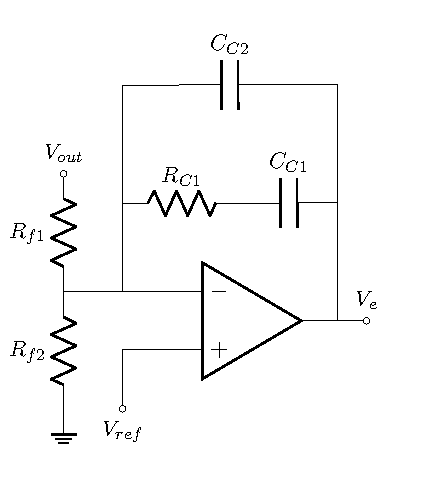
\includegraphics[width=0.3\linewidth, page = 1]{ImagenesParteIII/CircuitsP3.pdf}
	\label{fig:compensador}
	\caption{Circuito compensador del sistema.}
\end{figure}

La transferencia de este sistema es la siguiente:
\begin{equation}
	H(s) = \frac{ 1 }{ R_{f1} C_{C2} } \cdot \frac{s + \frac{1}{ R_{C1} C_{C1}}}{ s \left( s + \frac{R_{C1} + R_{C2}}{R_{C1} C_{C1} C_{C2}} \right)}
\end{equation}

Se emplean los siguientes valores:
\begin{multicols}{2}
\begin{itemize}
	\item $R_{C1} = 10 \ k\Omega$
	\item $R_{f1} = R_{f2} = 1 \ k\Omega$
	\item $C_{C1} = 10 \ nf$
	\item $C_{C2} = 1 \ \mu f$
	\item $N_2 = 1 \ \mu H$
\end{itemize}
\end{multicols}

Con esos valores, el compensador queda:
\begin{equation}
	H(s) = \frac{0.0001 s + 1}{ 1 \cdot 10^{-7} s^2 + 0.00101 s }
\end{equation}

Con el sistema realimentado, se grafican los diagramas de Bode para la transferencia y para la ganancia de lazo T, algiual que el diagrama de polos y ceros del sistema.
\begin{figure}[H]
	\centering
	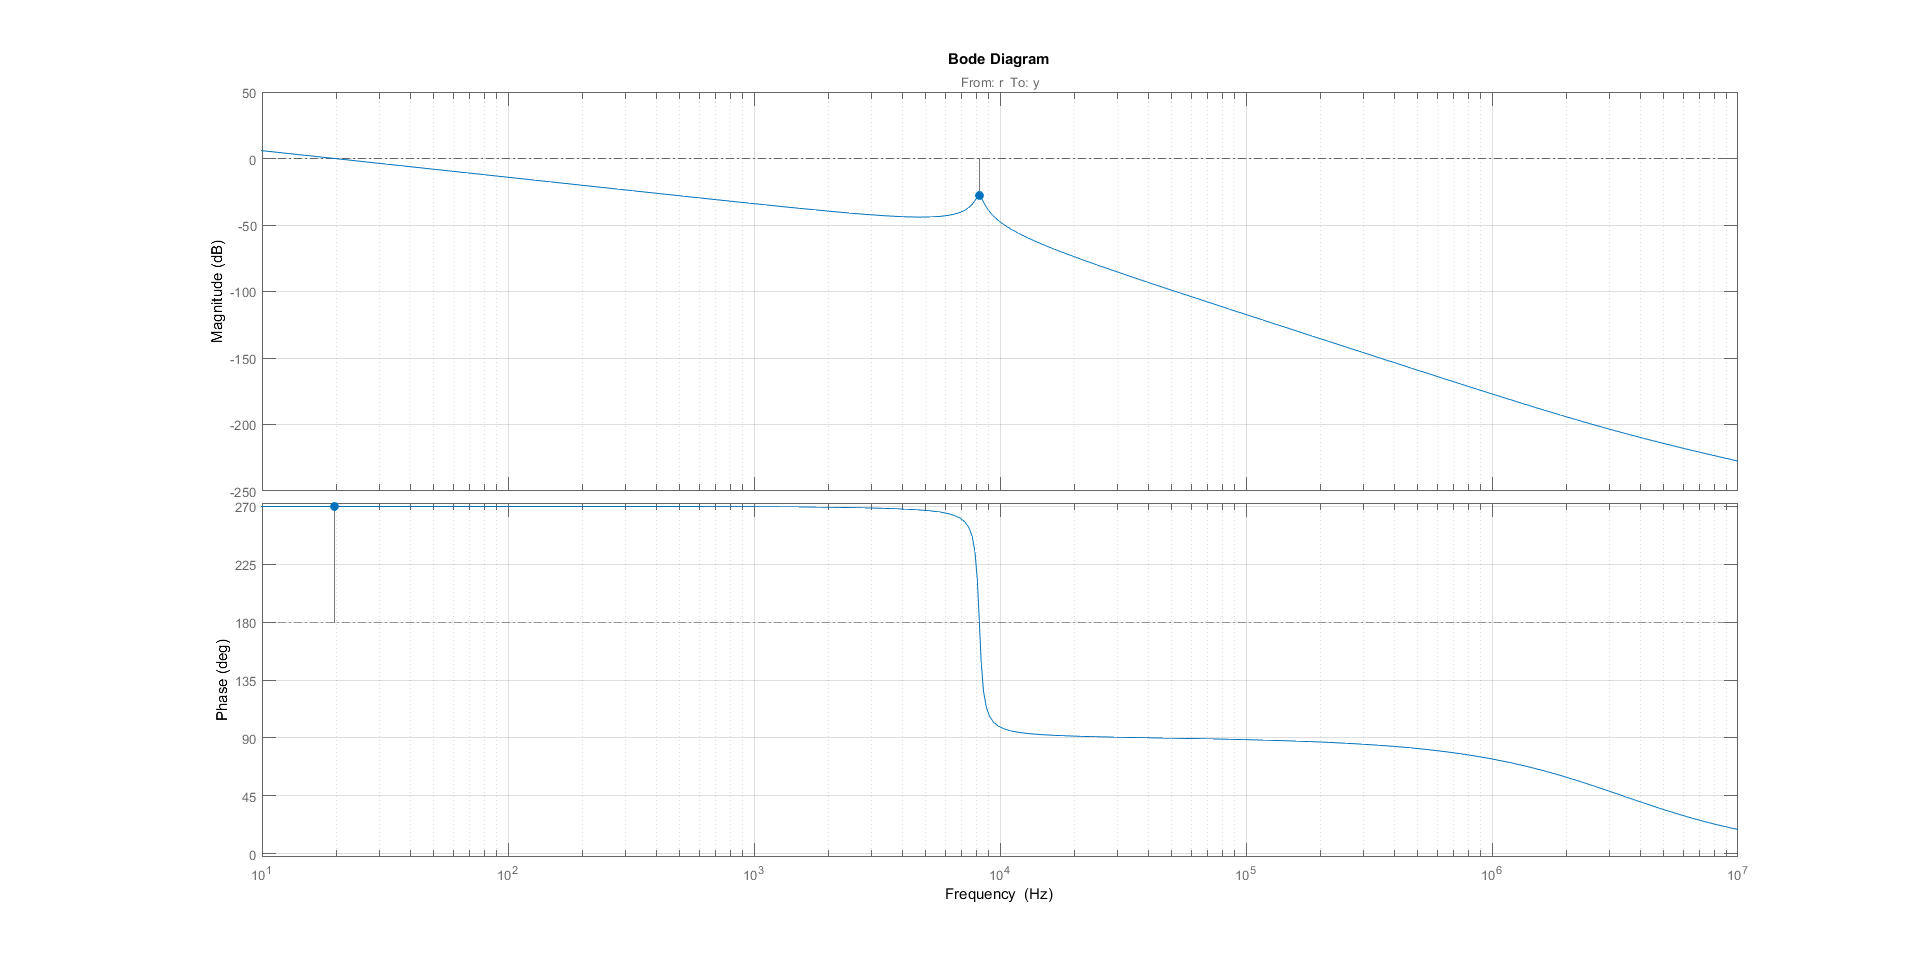
\includegraphics[width=0.9\linewidth]{ImagenesParteIII/Bode.png}
	\label{fig:bode}
	\caption{Diagrama de Bode transferencia.}
\end{figure}
\begin{figure}[H]
	\centering
	\includegraphics[width=0.9\linewidth]{ImagenesParteIII/BodeT.png}
	\label{fig:bodeT}
	\caption{Diagrama de Bode ganancia de lazo.}
\end{figure}

\begin{figure}[H]
	\centering
	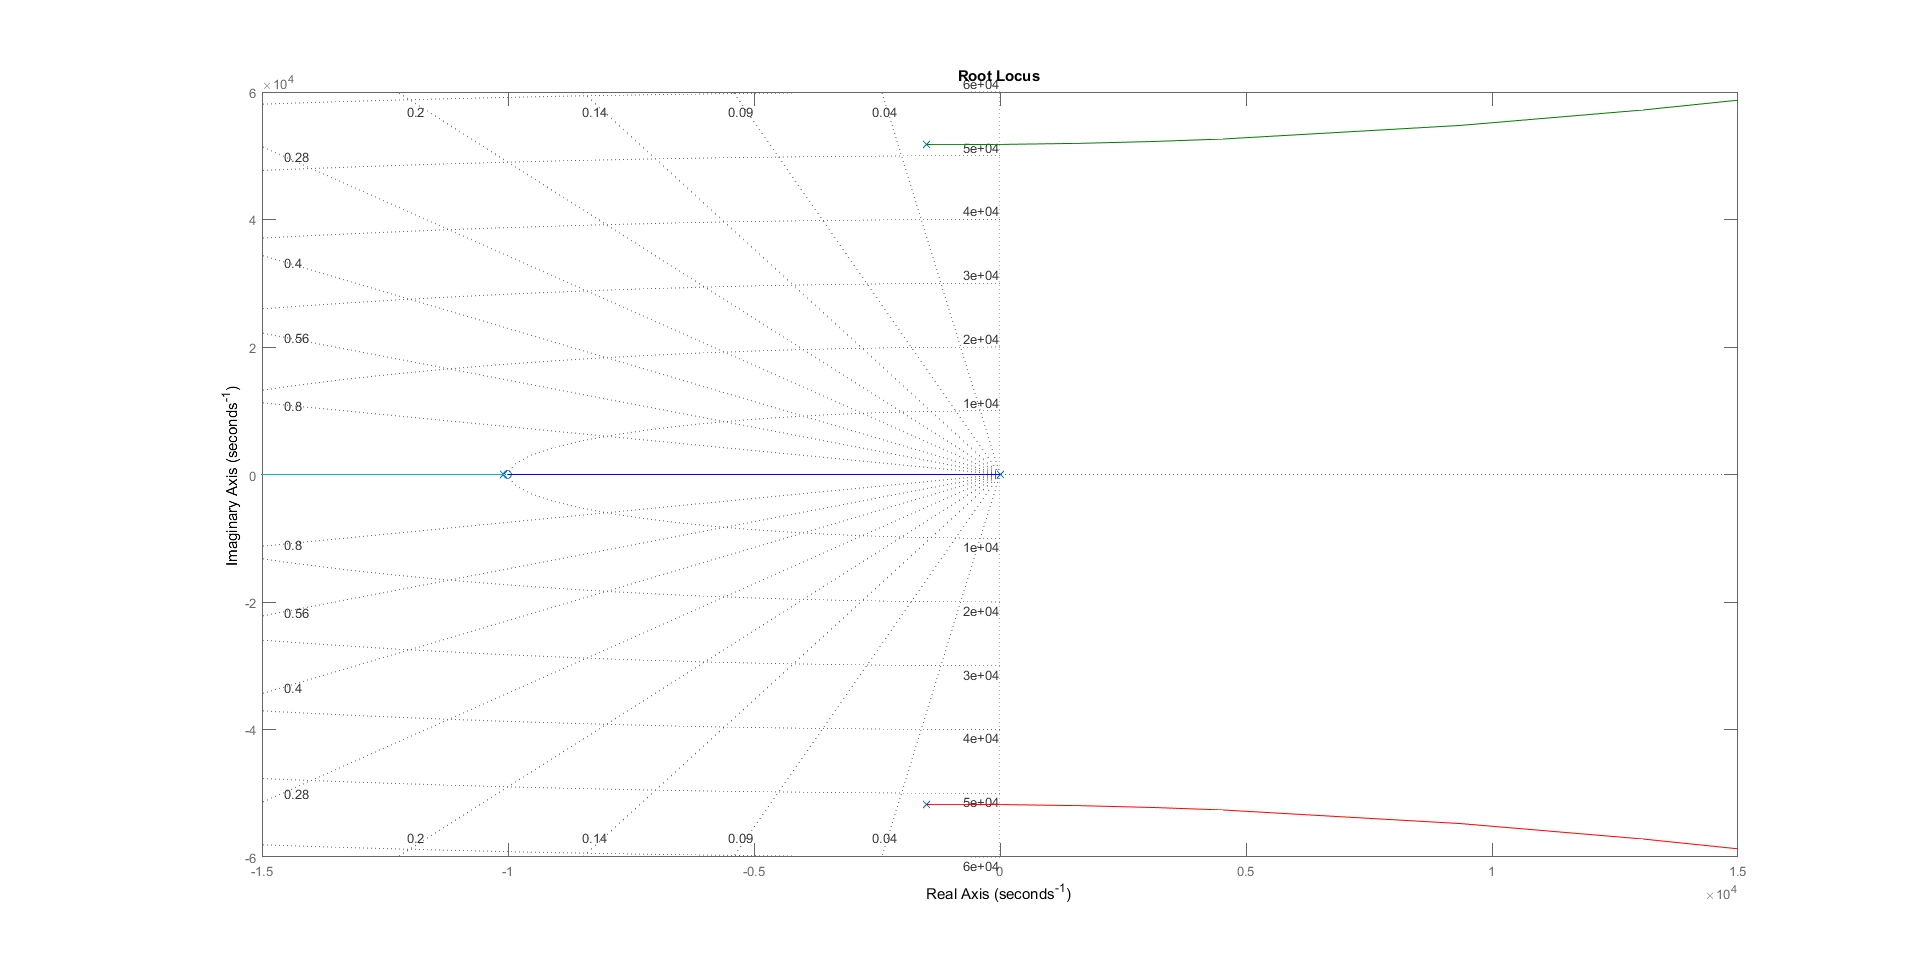
\includegraphics[width=0.9\linewidth]{ImagenesParteIII/Rlocus.png}
	\label{fig:zplane}
	\caption{Plano S, diagrama de polos y ceros.}
\end{figure}
En lineas generales, si 
\begin{equation}
|T| >> 1 \implies \ \frac{V_o}{V_{ref}} \approx \frac{1}{\beta} =  0.5 \ \implies V_o\approx 0.5 \cdot V_{ref} 
\end{equation}

En el diseño del realimentador se tuvieron en cuenta diversos lugares para colocar una resistencia variable. Esta podría ser en $R_{f1}$, $R_{f2}$ o simplemente se podría variar la $V_{ref}$.

El problema que se encontró con poner la variable en $R_{f2}$ es que la variación de salida con esta resistencia resulta homográfica, siendo preferible que sea lineal. Es por ello que esta opción quedó descartada. Finalmente se optó por variar únicamente la tension de $V_{ref}$.

Debido a que los potenciómetros cuentan con una inductancia parásita considerable y, dado que este es el realimentador, se podrían introducir polos ó ceros indeseados al sistema empleando dicho componente.
 
Finalmente se realizó la simulación a lazo cerrado y se obtuvieron las siguientes curvas:

\begin{figure}[H]
	\centering
	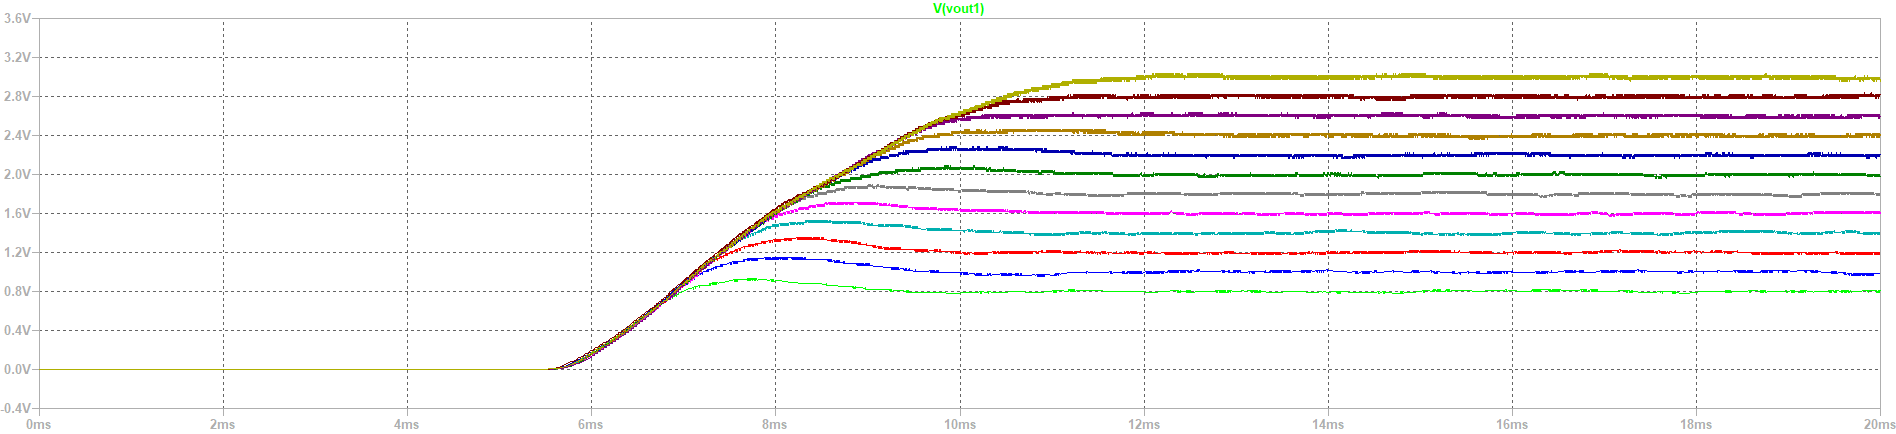
\includegraphics[width=0.9\linewidth]{ImagenesParteIII/Vouts.png}
	\label{fig:vouts_3}
	\caption{Variación de tensión de salida.}
\end{figure}
%\end{document}